% Author: Paul Shao
% Email: paulshaoyuqiao1@berkeley.edu
In discussion, we talked about rotation matrix as an example of transformation on a given vector. 

A rotation matrix is a matrix that takes a vector and rotates it by some number of degrees (counter-clockwise). That matrix looks like: \\
  $$\begin{bmatrix}
  \cos{\theta} & -\sin{\theta} \\
  \sin{\theta} & \cos{\theta} \end{bmatrix}$$ \\

  for some angle $\theta$. 

  In this question, we will explore some of the properties a rotation matrix has in more depth and see how the algebra behind is deeply connected to the geometric transformation we see.

  \note{
    Before proceeding, please show the students how the rotation matrix is actually derived. Especially show them how it is a linear transformation on the two following vectors in the standard basis of $\mathbb{R}^2$:
    $$\vec{e}_1 = \begin{bmatrix}
      1 \\ 0
    \end{bmatrix}, \:\: \vec{e}_2 = \begin{bmatrix}
      0 \\ 1
    \end{bmatrix}$$
    Here's an accompanying figure that helps illustrate the process:
    \begin{figure}[H]
      \centering
      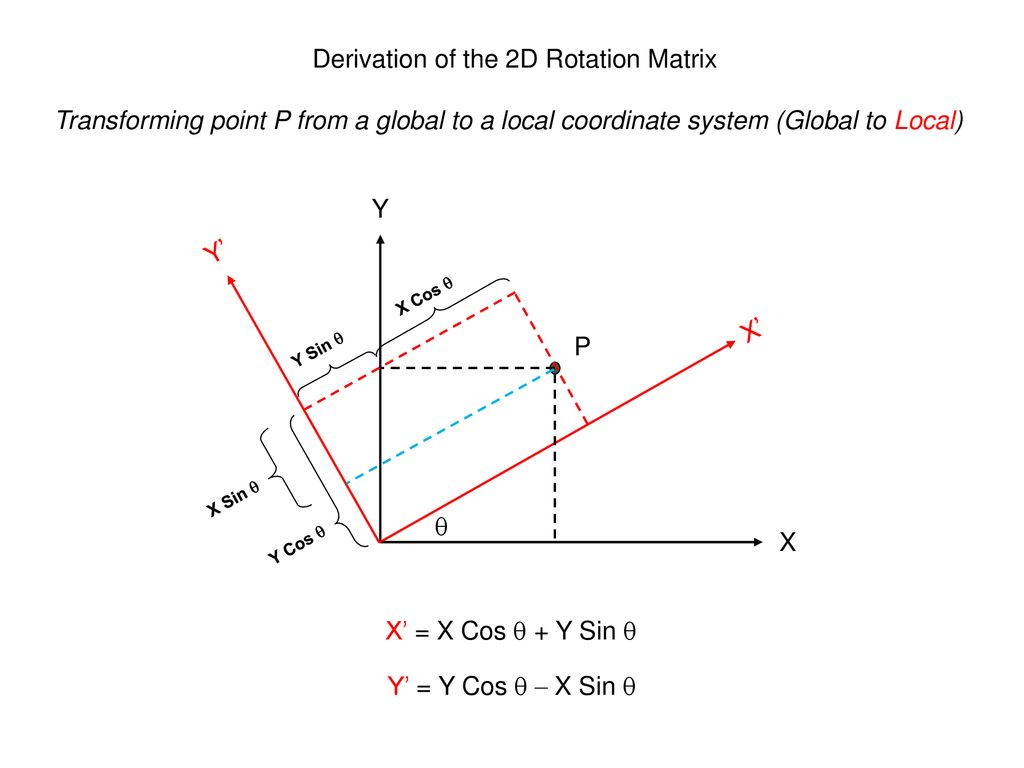
\includegraphics[width=14cm]{../rotation.png}
    \end{figure}
  }

  \begin{enumerate}
      \item Given the following vector: 
      $$\vec{v} = \begin{bmatrix}
0\\
1
\end{bmatrix}$$
    If we want to rotate $\vec{v}$ counter-clockwise by $\theta = 45^o$, what would the rotation matrix corresponding to this transformation be? What would the resulting vector be?
    
    \note{For this question, it might be helpful to plot out the vector on a 2D coordinate system on the board and first discuss with the students on what the rotation process would look like. It is also a good idea to review some trigonometry with the students in case they weren't as familiar with the notation.}
    
    \sol{Since $\theta = 45$ degrees, we can plug $\theta$ directly into the given rotation matrix above.
    $$R = \begin{bmatrix}
  \cos{\theta} & -\sin{\theta} \\
  \sin{\theta} & \cos{\theta} \end{bmatrix} = \begin{bmatrix}
  \cos{45^o} & -\sin{45^o} \\
  \sin{45^o} & \cos{45^o} \end{bmatrix} = \begin{bmatrix}
  \frac{\sqrt{2}}{2} & -\frac{\sqrt{2}}{2} \\
  \frac{\sqrt{2}}{2} & \frac{\sqrt{2}}{2} \end{bmatrix}$$
    
    To find the resulting vector, we can either plot the rotated vector out on a 2D grid and use trigonometry to determine the new coordinates of the vector; or we can directly multiply $\vec{v}$ by the rotation matrix (as a transformation):
    $$\vec{v_{rotated}} = R\vec{v} = \begin{bmatrix}
-\frac{\sqrt{2}}{2}\\ 
\frac{\sqrt{2}}{2}
\end{bmatrix}$$
}
\item In this part, we will explore the relationship between a series of counter-clockwise rotations applied on a given vector and how the rotation matrix is represented correspondingly. 

Given that we have found the rotation matrix $R$ for $\theta = 45^o$ in the previous part, now find the rotation matrix for $\theta = 90^o$, $\theta = 135^o$. At the same time, evaluate the matrix product $R^2, R^3$. What pattern did you see?

\note{For this question, since we are dealing with matrix multiplication with entries involving square roots, make sure to walk the students through a demo of the calculation. At the same time, encourage the students to think visually in terms of repeatedly rotating the vector on the 2D grid.}

\sol{Following the same steps in part (a), we can directly plug $\theta = 90^o$ and $\theta = 135^o$ into the given rotation matrix expression. Let the 90-degrees rotation matrix be $R_2$, and let the 135 degrees rotation matrix be $R_3$. We have:
  $$R_2 = \begin{bmatrix}
  0 & -1 \\
  1 & 0 \end{bmatrix}$$
    $$R_3 = \begin{bmatrix}
  -\frac{\sqrt{2}}{2} & -\frac{\sqrt{2}}{2} \\
  \frac{\sqrt{2}}{2} & -\frac{\sqrt{2}}{2} \end{bmatrix}$$
  At the same time, if we evaluate $R^2$ and $R^3$, where $R$ is the 45-degrees rotation matrix, we will find out that 
  $R_2 = R^2$ and $R_3 = R^3$! 
  
  What this really means, from an intuitive standpoint, is that we can represent the rotation transformation with the rotation matrix. What's more, a 90-degrees rotation can be replaced with two 45-degrees rotation, and a 135-degrees rotation can be replaced with three 45-degrees rotation, and so forth! The multiplication of the rotation matrix continuously applies the rotation transformation on the actual vector. 
}
\item Generalizing from the previous part, if we are given a rotation matrix $M$ that rotates a given vector $\vec{v}$ by $k$ degrees. What would the resulting vector $\vec{v}'$ be if we rotate $\vec{v}$ by a total of $N \times k$ degrees? ($N$ is a positive integer).

\note{To help students cope with the more generalized and symbolic notation, it might be helpful to begin again with numerical examples from the previous part and then extend to $\theta = 180^o$, $\theta = 225^o$, $\dots$ to show more concrete patterns.} 

\sol{As we have seen from the previous part, every time a rotation is applied, we can equivalent multiply the original vector by the corresponding rotation matrix.

In this case, since we are rotating by a total of $N \times k$ degrees, and we know of a rotation matrix that rotates a given vector by $k$ degrees, we can view it as applying the $k$-degrees rotation a total of $N$ times. 

Hence, this will lead us to the following expression for the resulting vector:
$$\vec{v}' = M^N \vec{v}$$
}
\item Backing off from counter-clockwise rotation for a bit, let's now explore \textbf{clockwise rotation} instead on a given vector.  Given the \textbf{counter-clockwise rotation} matrix $R_{c}$ we provided at the beginning of the question, consider the rotation matrix $R_{c'}$ for a \textbf{clockwise rotation} of $\theta$ degrees. What is the relationship between $R_{c'}$ and $R_{c}$?

\note{Encourage the students to think intuitively about this question. Direct them especially at the key point where clockwise rotation is a reverse process of the counter-clockwise rotation. Bonus points if the students also realize that a clockwise rotation by $\theta$ is simply a counter-clockwise rotation with $360n - \theta$ degrees (complements of each other)}

\sol{As we can see, clockwise rotation is counter-clockwise rotation but backwards! What that really means is that, if we apply a counter-clockwise rotation matrix to a given vector, we can apply a clockwise rotation matrix to \textbf{reverse} that process. 

With that being said, we have learned in class that a transformation matrix that can \textbf{undo} a previous transformation $T$ is its inverse $T^{-1}$.

Hence, $R_{c'}$ and $R_{c}$ are inverses of each other!}

\item Now that we have learned about the intrinsic connections between rotation matrix multiplication/inverse and the geometric transformation, in a few sentences, explain why the multiplication of rotation matrices is commutative. i.e.: Explain why given two rotation matrices $A$ and $B$ ($A$ and $B$ are both $N \times N$) , $AB = BA$.

\note{Encourage the students to think in terms of the overall resulting vector and contrast that with the order of our rotation.

{
  \color{NavyBlue}
  It is \textbf{EXTREMELY CRUCIAL} to emphasize to the students that the reason we can conclude $AB = BA$ in the end is because $\vec{v}$ can be any vector from $\mathbb{R}^2$. \\ \\
  The implication (out of scope for this class) is because we can see that $$Nul(AB - BA) = \mathbb{R}^2,$$ and by the fundamental theorem of linear algebra, $$Col(AB - BA) \: \oplus \: Nul(AB - BA) = \mathbb{R}^2,$$ this tells us that $$Col(AB - BA) = \{ \vec{0} \}.$$
  The justification above is \textbf{NON-TRIVIAL}, and you cannot conclude $AB - BA = 0$ without having $\vec{v}$ being any vector from $\mathbb{R}^2$!!!
}
}

\sol{Geometrically, since we are rotating the vector by the sum of all the given degrees from the rotation matrices. It doesn't matter how many degrees we rotate the vector first during the process.

Hence, we can conclude that for any given vector $\vec{v}$:
$$AB\vec{v} = BA\vec{v}$$
$$(AB-BA)\vec{v} = 0$$
Since $\vec{v}$ could be any vectors in $\mathbb{R}^2$, we know that it must be true that $AB - BA = 0$, and therefore $AB = BA$.
}

\item Finally, for one additional nice property that results from rotation matrix multiplication, we know that if we rotate a vector each time by 30 degrees for a total of 12 times, eventually it will be a total of 360 degrees rotation, which puts the vector right back to where it was originally! Utilizing this fact, find a $2 \times 2$ matrix $M$ such that $M^7 = I$, where $I$ is the identity matrix.

\note{Encourage the students to directly associate matrix multiplication with rotation transformation. Also, utilize the fact that a rotation of a multiple of 360 degrees is equivalent to not rotating at all, which returns the $\textbf{same and original}$ vector.}

\sol{We can treat the identity matrix as geometrically not touching a given vector at all (just leaving it as it is). Since we know that a 360 degrees rotation will reset the vector back to itself, we know that it is also equivalent to applying the identity matrix to that vector. Given this information, we can now reword our question as follows:

Given a rotation matrix $M$ that rotates a vector $\vec{v}$ by a total of 7 times (this comes from $M^7$), each time by $x$ degrees, what should $x$ be such that $7x$ is equal to some multiples of 360?

Now, this becomes a much simpler algebra question. For ease of computation, we can pick 360 as one of the multiples. This will give us the equation:
$$7x = 360^{\circ}$$
Solving for $x$, we have $x = 360/7^{\circ}$. Hence, we know that if we apply a rotation matrix that rotates a vector by $360/7$ degrees for a total of 7 times, it will be equivalent to leaving the vector as it is!

Hence, $M$ = the rotation matrix with $\theta = 360/7^{^\circ}$.}

  \end{enumerate}